% Options for packages loaded elsewhere
\PassOptionsToPackage{unicode}{hyperref}
\PassOptionsToPackage{hyphens}{url}
%
\documentclass[
]{article}
\usepackage{lmodern}
\usepackage{amssymb,amsmath}
\usepackage{ifxetex,ifluatex}
\ifnum 0\ifxetex 1\fi\ifluatex 1\fi=0 % if pdftex
  \usepackage[T1]{fontenc}
  \usepackage[utf8]{inputenc}
  \usepackage{textcomp} % provide euro and other symbols
\else % if luatex or xetex
  \usepackage{unicode-math}
  \defaultfontfeatures{Scale=MatchLowercase}
  \defaultfontfeatures[\rmfamily]{Ligatures=TeX,Scale=1}
\fi
% Use upquote if available, for straight quotes in verbatim environments
\IfFileExists{upquote.sty}{\usepackage{upquote}}{}
\IfFileExists{microtype.sty}{% use microtype if available
  \usepackage[]{microtype}
  \UseMicrotypeSet[protrusion]{basicmath} % disable protrusion for tt fonts
}{}
\makeatletter
\@ifundefined{KOMAClassName}{% if non-KOMA class
  \IfFileExists{parskip.sty}{%
    \usepackage{parskip}
  }{% else
    \setlength{\parindent}{0pt}
    \setlength{\parskip}{6pt plus 2pt minus 1pt}}
}{% if KOMA class
  \KOMAoptions{parskip=half}}
\makeatother
\usepackage{xcolor}
\IfFileExists{xurl.sty}{\usepackage{xurl}}{} % add URL line breaks if available
\IfFileExists{bookmark.sty}{\usepackage{bookmark}}{\usepackage{hyperref}}
\hypersetup{
  pdftitle={Statistical analysis in RStudio},
  hidelinks,
  pdfcreator={LaTeX via pandoc}}
\urlstyle{same} % disable monospaced font for URLs
\usepackage[margin=1in]{geometry}
\usepackage{longtable,booktabs}
% Correct order of tables after \paragraph or \subparagraph
\usepackage{etoolbox}
\makeatletter
\patchcmd\longtable{\par}{\if@noskipsec\mbox{}\fi\par}{}{}
\makeatother
% Allow footnotes in longtable head/foot
\IfFileExists{footnotehyper.sty}{\usepackage{footnotehyper}}{\usepackage{footnote}}
\makesavenoteenv{longtable}
\usepackage{graphicx,grffile}
\makeatletter
\def\maxwidth{\ifdim\Gin@nat@width>\linewidth\linewidth\else\Gin@nat@width\fi}
\def\maxheight{\ifdim\Gin@nat@height>\textheight\textheight\else\Gin@nat@height\fi}
\makeatother
% Scale images if necessary, so that they will not overflow the page
% margins by default, and it is still possible to overwrite the defaults
% using explicit options in \includegraphics[width, height, ...]{}
\setkeys{Gin}{width=\maxwidth,height=\maxheight,keepaspectratio}
% Set default figure placement to htbp
\makeatletter
\def\fps@figure{htbp}
\makeatother
\setlength{\emergencystretch}{3em} % prevent overfull lines
\providecommand{\tightlist}{%
  \setlength{\itemsep}{0pt}\setlength{\parskip}{0pt}}
\setcounter{secnumdepth}{5}
\usepackage{subfig}

\title{Statistical analysis in RStudio}
\author{}
\date{\vspace{-2.5em}}

\begin{document}
\maketitle

{
\setcounter{tocdepth}{2}
\tableofcontents
}
\hypertarget{abstact}{%
\subsubsection{Abstact}\label{abstact}}

\hypertarget{introduction}{%
\section{INTRODUCTION}\label{introduction}}

\begin{longtable}[]{@{}llllr@{}}
\toprule
Summer & Year.Month & Site & Species & average.count\tabularnewline
\midrule
\endhead
summer-2007 & 2007.Jun & A & HARBOUR & 14.1\tabularnewline
summer-2007 & 2007.Jun & B & HARBOUR & 0.3\tabularnewline
summer-2007 & 2007.Jun & C & HARBOUR & 14.7\tabularnewline
summer-2007 & 2007.Jun & Spit & HARBOUR & 0.1\tabularnewline
summer-2007 & 2007.Jun & Wall & HARBOUR & 0.7\tabularnewline
summer-2007 & 2007.Jun & D & HARBOUR & 0.0\tabularnewline
\bottomrule
\end{longtable}

\begin{verbatim}
## 'data.frame':    210 obs. of  5 variables:
##  $ Summer       : chr  "summer-2007" "summer-2007" "summer-2007" "summer-2007" ...
##  $ Year.Month   : chr  "2007.Jun" "2007.Jun" "2007.Jun" "2007.Jun" ...
##  $ Site         : chr  "A" "B" "C" "Spit" ...
##  $ Species      : chr  "HARBOUR" "HARBOUR" "HARBOUR" "HARBOUR" ...
##  $ average.count: num  14.1 0.3 14.7 0.1 0.7 0 0 0.3 0 2.6 ...
\end{verbatim}

\begin{verbatim}
## 'data.frame':    210 obs. of  5 variables:
##  $ Summer       : Factor w/ 4 levels "2007","2008",..: 1 1 1 1 1 1 1 1 1 1 ...
##  $ Year.Month   : Factor w/ 15 levels "2007.Aug","2007.Jul",..: 3 3 3 3 3 3 3 3 3 3 ...
##  $ Site         : Factor w/ 7 levels "A","B","C","D",..: 1 2 3 6 7 4 5 1 2 3 ...
##  $ Species      : Factor w/ 2 levels "GREY","HARBOUR": 2 2 2 2 2 2 2 1 1 1 ...
##  $ average.count: num  14.1 0.3 14.7 0.1 0.7 0 0 0.3 0 2.6 ...
\end{verbatim}

\hypertarget{materials-and-methods}{%
\section{MATERIALS AND METHODS}\label{materials-and-methods}}

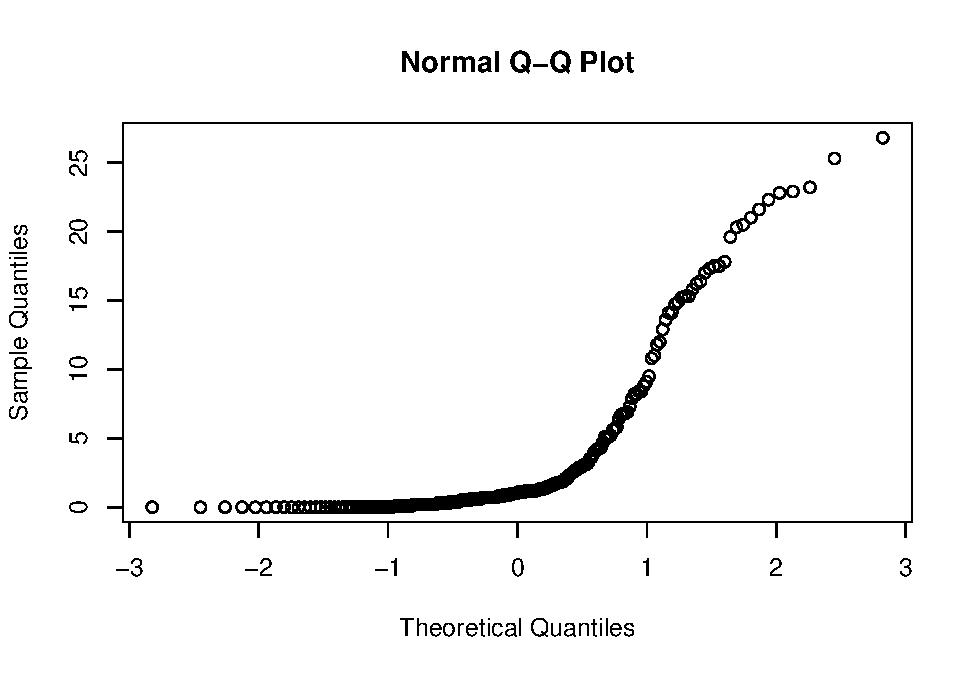
\includegraphics{Statistical-analysis-in-RStudio_files/figure-latex/unnamed-chunk-5-1.pdf}

\begin{verbatim}
## 
##  Shapiro-Wilk normality test
## 
## data:  data$average.count
## W = 0.67749, p-value < 2.2e-16
\end{verbatim}

\begin{verbatim}
## 
##  Kruskal-Wallis rank sum test
## 
## data:  data$average.count and data$Summer
## Kruskal-Wallis chi-squared = 6.236, df = 3, p-value = 0.1007
\end{verbatim}

\begin{verbatim}
## 
##  Pairwise comparisons using Wilcoxon rank sum test with continuity correction 
## 
## data:  data$average.count and data$Summer 
## 
##      2007 2008 2009
## 2008 0.89 -    -   
## 2009 0.20 0.43 -   
## 2010 0.43 0.64 0.89
## 
## P value adjustment method: holm
\end{verbatim}

\begin{verbatim}
## 
##  Pairwise comparisons using Wilcoxon rank sum test with continuity correction 
## 
## data:  data$average.count and data$Summer 
## 
##      2007 2008 2009
## 2008 0.54 -    -   
## 2009 0.17 0.17 -   
## 2010 0.17 0.32 0.75
## 
## P value adjustment method: BH
\end{verbatim}

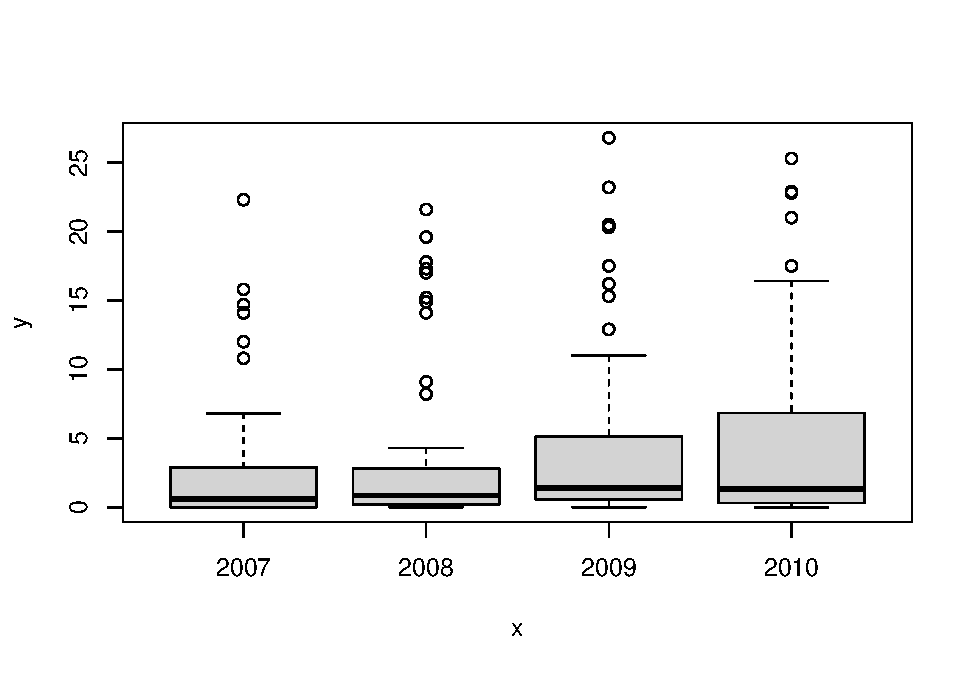
\includegraphics{Statistical-analysis-in-RStudio_files/figure-latex/unnamed-chunk-10-1.pdf}

\begin{verbatim}
## 
##  Kruskal-Wallis rank sum test
## 
## data:  data$average.count[data$Summer == "2007"] and data$Year.Month[data$Summer == "2007"]
## Kruskal-Wallis chi-squared = 1.3113, df = 2, p-value = 0.5191
\end{verbatim}

\begin{verbatim}
## Warning in wilcox.test.default(xi, xj, paired = paired, ...): cannot compute
## exact p-value with ties

## Warning in wilcox.test.default(xi, xj, paired = paired, ...): cannot compute
## exact p-value with ties

## Warning in wilcox.test.default(xi, xj, paired = paired, ...): cannot compute
## exact p-value with ties
\end{verbatim}

\begin{verbatim}
## 
##  Pairwise comparisons using Wilcoxon rank sum test with continuity correction 
## 
## data:  data$average.count[data$Summer == "2007"] and data$Year.Month[data$Summer == "2007"] 
## 
##          2007.Aug 2007.Jul
## 2007.Jul 0.63     -       
## 2007.Jun 0.63     0.63    
## 
## P value adjustment method: BH
\end{verbatim}

\begin{verbatim}
## 
##  Kruskal-Wallis rank sum test
## 
## data:  data$average.count and data$Species
## Kruskal-Wallis chi-squared = 18.66, df = 1, p-value = 1.562e-05
\end{verbatim}

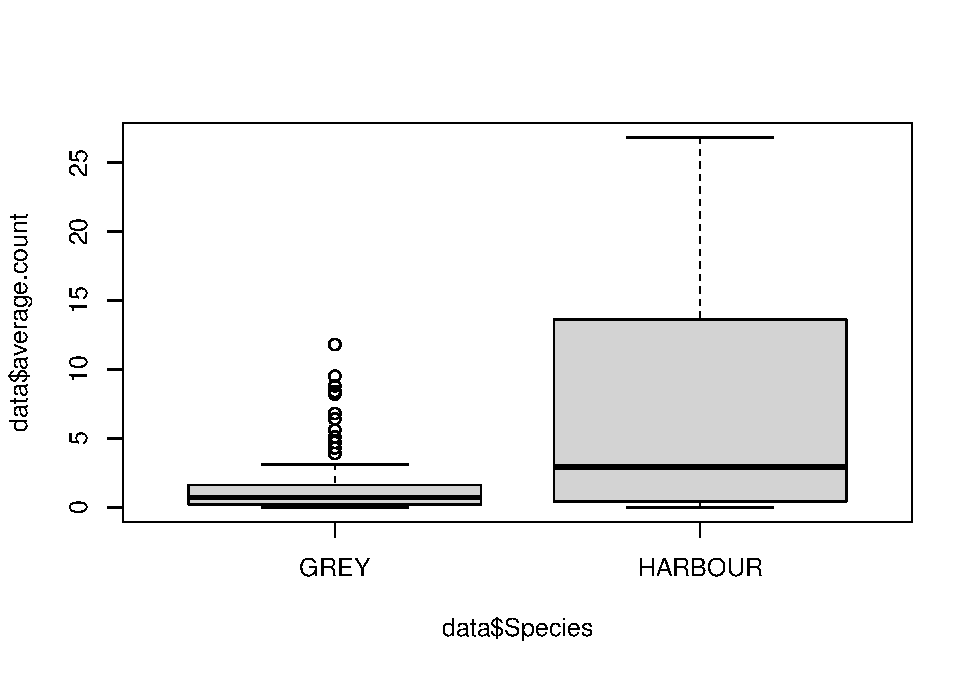
\includegraphics{Statistical-analysis-in-RStudio_files/figure-latex/unnamed-chunk-14-1.pdf}

\begin{verbatim}
## 
##  Kruskal-Wallis rank sum test
## 
## data:  data$average.count and data$Species
## Kruskal-Wallis chi-squared = 18.66, df = 1, p-value = 1.562e-05
\end{verbatim}

\begin{verbatim}
## 
##  Pairwise comparisons using Wilcoxon rank sum test with continuity correction 
## 
## data:  data$average.count and data$Species 
## 
##         GREY   
## HARBOUR 1.6e-05
## 
## P value adjustment method: BH
\end{verbatim}

\begin{verbatim}
## 
##  Kruskal-Wallis rank sum test
## 
## data:  data$average.count[data$Summer == "2007"] and data$Species[data$Summer == "2007"]
## Kruskal-Wallis chi-squared = 3.2976, df = 1, p-value = 0.06938
\end{verbatim}

\begin{verbatim}
## Warning in wilcox.test.default(xi, xj, paired = paired, ...): cannot compute
## exact p-value with ties
\end{verbatim}

\begin{verbatim}
## 
##  Pairwise comparisons using Wilcoxon rank sum test with continuity correction 
## 
## data:  data$average.count[data$Summer == "2007"] and data$Species[data$Summer == "2007"] 
## 
##         GREY 
## HARBOUR 0.071
## 
## P value adjustment method: BH
\end{verbatim}

\begin{verbatim}
## 
##  Kruskal-Wallis rank sum test
## 
## data:  data$average.count[data$Summer == "2008"] and data$Species[data$Summer == "2008"]
## Kruskal-Wallis chi-squared = 2.727, df = 1, p-value = 0.09866
\end{verbatim}

\begin{verbatim}
## Warning in wilcox.test.default(xi, xj, paired = paired, ...): cannot compute
## exact p-value with ties
\end{verbatim}

\begin{verbatim}
## 
##  Pairwise comparisons using Wilcoxon rank sum test with continuity correction 
## 
## data:  data$average.count[data$Summer == "2008"] and data$Species[data$Summer == "2008"] 
## 
##         GREY
## HARBOUR 0.1 
## 
## P value adjustment method: BH
\end{verbatim}

\begin{verbatim}
## 
##  Kruskal-Wallis rank sum test
## 
## data:  data$average.count[data$Summer == "2009"] and data$Species[data$Summer == "2009"]
## Kruskal-Wallis chi-squared = 10.332, df = 1, p-value = 0.001307
\end{verbatim}

\begin{verbatim}
## Warning in wilcox.test.default(xi, xj, paired = paired, ...): cannot compute
## exact p-value with ties
\end{verbatim}

\begin{verbatim}
## 
##  Pairwise comparisons using Wilcoxon rank sum test with continuity correction 
## 
## data:  data$average.count[data$Summer == "2009"] and data$Species[data$Summer == "2009"] 
## 
##         GREY  
## HARBOUR 0.0013
## 
## P value adjustment method: BH
\end{verbatim}

\begin{verbatim}
## 
##  Kruskal-Wallis rank sum test
## 
## data:  data$average.count[data$Summer == "2010"] and data$Species[data$Summer == "2010"]
## Kruskal-Wallis chi-squared = 4.1213, df = 1, p-value = 0.04235
\end{verbatim}

\begin{verbatim}
## Warning in wilcox.test.default(xi, xj, paired = paired, ...): cannot compute
## exact p-value with ties
\end{verbatim}

\begin{verbatim}
## 
##  Pairwise comparisons using Wilcoxon rank sum test with continuity correction 
## 
## data:  data$average.count[data$Summer == "2010"] and data$Species[data$Summer == "2010"] 
## 
##         GREY 
## HARBOUR 0.043
## 
## P value adjustment method: BH
\end{verbatim}

\hypertarget{results}{%
\section{RESULTS}\label{results}}

\hypertarget{discussion}{%
\section{DISCUSSION}\label{discussion}}

\hypertarget{references}{%
\subsubsection{REFERENCES}\label{references}}

\end{document}
